\section{One Variable Integral Calculus}

\subsection{The Mercator Map and the Integral of Secant}

\subsubsection*{Historical Motivation}

A great reference for the history of the integral of the secant function and its relation to the Mercator map is \cite{mercator}. We will give a brief overview here.

The Mercator Map of the world spaces out the lines of latitude in a particular way inorder to solve a problem in naval navigation. 
The problem is that ships would navigate by sailing with a fixed angle to due north (e.g. as seen on a compass). 
This creates an issue for making map. 
Consider a map where the lines of latitude are spaced out evenly in the vertical direction (so NOT the Mercator map); for such a map, a course with fixed angle to magnetic north is NOT a straight line on the map.  
The figure below shows the path of a course with constant angle to magnetic north on a map with uniformly spaced lines of latitude.

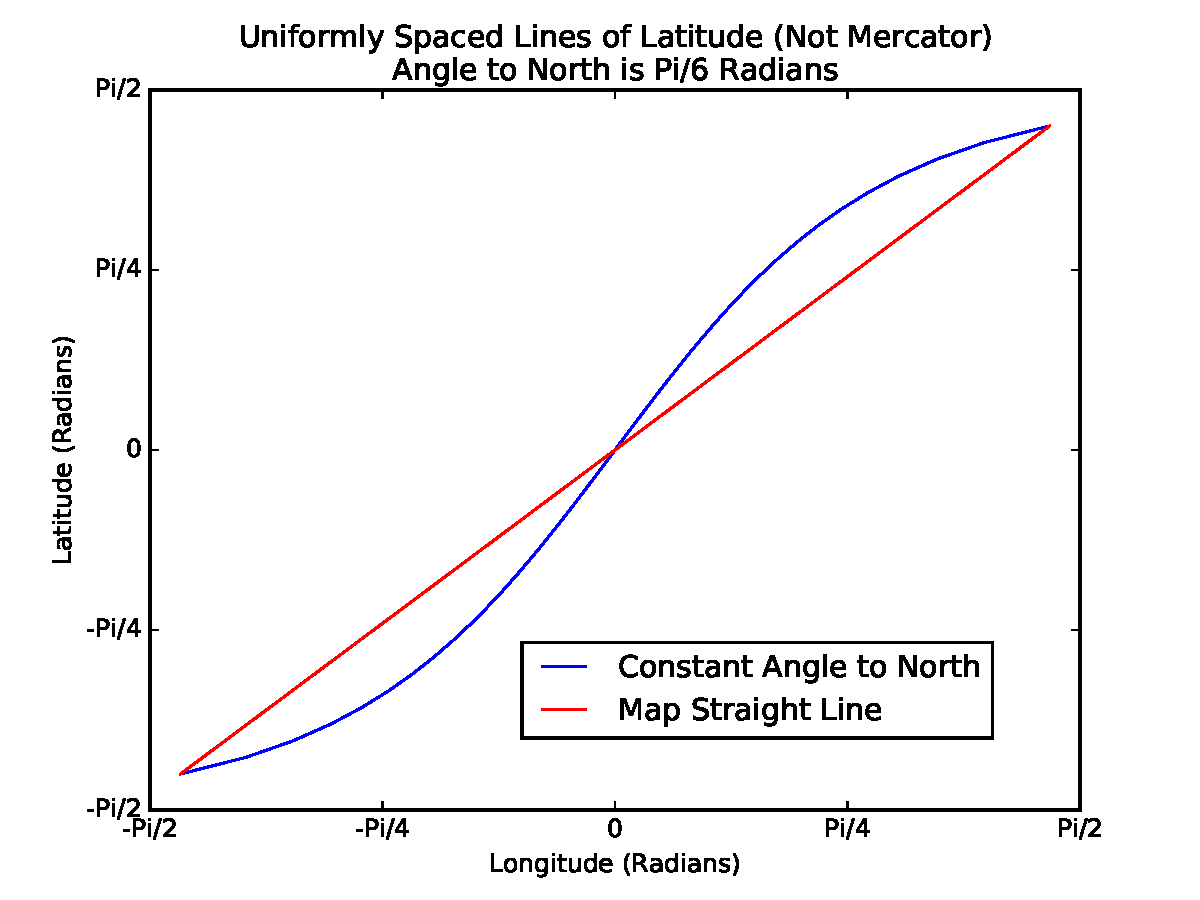
\includegraphics[width = 5in]{_generated/nonMercator.pdf}

The problem is that the lines of latitude get represent shorter and shorter distances as you move from the equator towards either of the poles. 
This means that there is a complicated relationship between the angle measured on this map and the true angle to magnetic north it represents.

In 1569, Mercator had the idea that he could create a map where the lines of latitude are NOT spaced evenly; if you choose the variation in spacing in the correct manner, then a course with fixed angle to magnetic north will be a straight line on this new map. 
Furthermore, the angle measured on the map will match the true angle to magnetic north.
Consider the following figure that shows a course with constant angle to magnetic north on a Mercator map, note that the lines of latitude are not evenly spaced (the values marked are multiples of \(\pi/9\) radians).

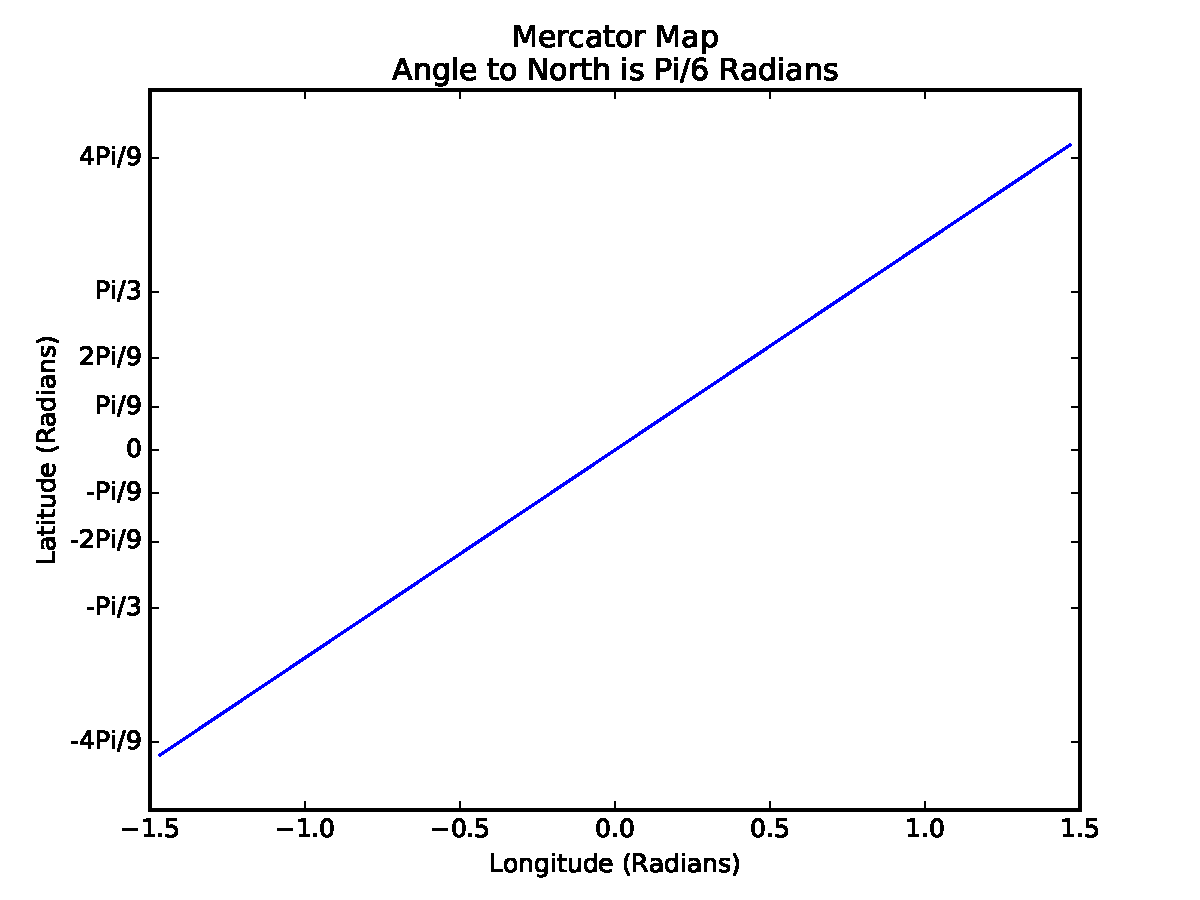
\includegraphics[width = 5in]{_generated/mercator.pdf}

Unfortunately, Mercator didn't give a clear formula to precisely describe how to space out the lines of latitude. 
However, in 1599, Edward Wright found a precise mathematical description of how to space out the lines; he found that the spacing depended on the area under the secant function.
He didn't know how to precisely compute this area, but he was able to approximate it. 

Later in the 1640's, Henry Bond looked at a table of these approximate areas and a table of logarithms of trigonometic functions. 
He noticed a similarity in the two tables, and he was able to conjecture a precise formula for the area under the secant function. 
We now know that his conjecture was correct, but at the time there was no proof beyond numerical tables.

A proof was later given by Isaac Barrow; this proof is the earliest known publication of the use of integration by partial fractions.

\subsubsection*{The Problem}

Compute the integral
\begin{equation}
\int\limits_0^x \sec(u) \du.
\end{equation}

\subsubsection*{The Solution}

Recall that \(\sec(u) = \frac{1}{\cos(u)}\). First, let's use algebraic manipulation combined with the trigonometric formula \(\cos^2(u) + \sin^2(u) = 1\).
\begin{align}
\int\limits_0^x \frac{1}{\cos(u)} \du & = \int\limits_0^x \frac{\cos(u)}{\cos^2(u)} \du, \\
    & = \int\limits_0^x \frac{\cos(u)}{1 - \sin^2(u)} \du.
\end{align}

Now, we do a \(u\)-substitution. However, we are already use the variable \(u\), so let's make it a "\(w\)-substitution". 
We use \(w = \sin(u)\), and so \(\dw = \cos(u) \du\). Then we have that our integral is:
\begin{equation}
\int\limits_0^{\sin(x)} \frac{1}{1 - w^2} \dw.
\end{equation}
 Now, we use partial fractions: 
\begin{align}
\frac{1}{1 - w^2} & = \frac{1}{(1 - w)(1 + w)},\\
    & = \frac{A}{1 - w} + \frac{B}{1 + w}.
\end{align}

Combining terms and comparing numerators, we get \(A + B + (A - B)w = 1\). So we have
\begin{equation}
\begin{cases}
A + B = 1, \\
A - B = 0.
\end{cases}
\end{equation}
Solving we get \(A = B = \frac{1}{2}\).

Therefore, our integral becomes
\begin{align}
\int\limits_0^{\sin(x)} \frac{1}{2(1 - w)} + \frac{1}{2(1 + w)} \dw 
    & = \left. \frac{1}{2} \log\left(\frac{1 + w}{1 - w}\right)\right|_0^{\sin(x)}, \\
    & = \frac{1}{2} \log\left(\frac{1 + \sin(x)}{1 - \sin(x)}\right).
\end{align}

To simplify things, we can now use some trigonometric identities.
\begin{align}
\frac{1}{2} \log\left(\frac{1 + \sin(x)}{1 - \sin(x)}\right) & = \log\sqrt{\frac{1 + \sin(x)}{1 - \sin(x)}}, \\
    & = \log\sqrt{\frac{(1 + \sin(x))^2}{1 - \sin^2(x)}}, \\
    & = \log\left(\frac{1 + \sin(x)}{\cos(x)}\right), \\
    & = \log(\sec(x) + \tan(x)).
\end{align}

%%%%%%%%%%%%%%%%%%%%%%%%%%%%%%%%%%%
%%%%%%% Fermat Method of Exhaustion
%%%%%%%%%%%%%%%%%%%%%%%%%%%%%%%%%%%

\subsection{Fermat's Method of Integrating Powers of \(x\)}

\subsubsection*{Motivation}

Consider the problem of finding the area underneath the curve for a particular power of \(x\); here we will concentrate on the 
particular case of \(y = x^{3/2}\) and \(0 \leq x \leq 1\). Note that the restriction of \(x\) to \(x\geq 0\) keeps everything well-defined within
the realm of real numbers. 

Before Leibniz and Newton developed the use of integral calculus to find the area under curves, Fermat had already developed 
a method to solve this particular problem. Let us put his idea into modern terms. His idea is to use a method of exhaustion to 
give lower bounds and upper bounds for the area. In particular, the key to his idea is that we will use rectangles whose widths
are not uniform. In fact, their widths decrease geometrically. 

For example, on the interval \(0 \leq x \leq 1\), one can bound the area above and below by the area of an infinite number of rectangles whose widths
are the powers of \(1/2\). To see this, consider the graph below for the lowerbound.

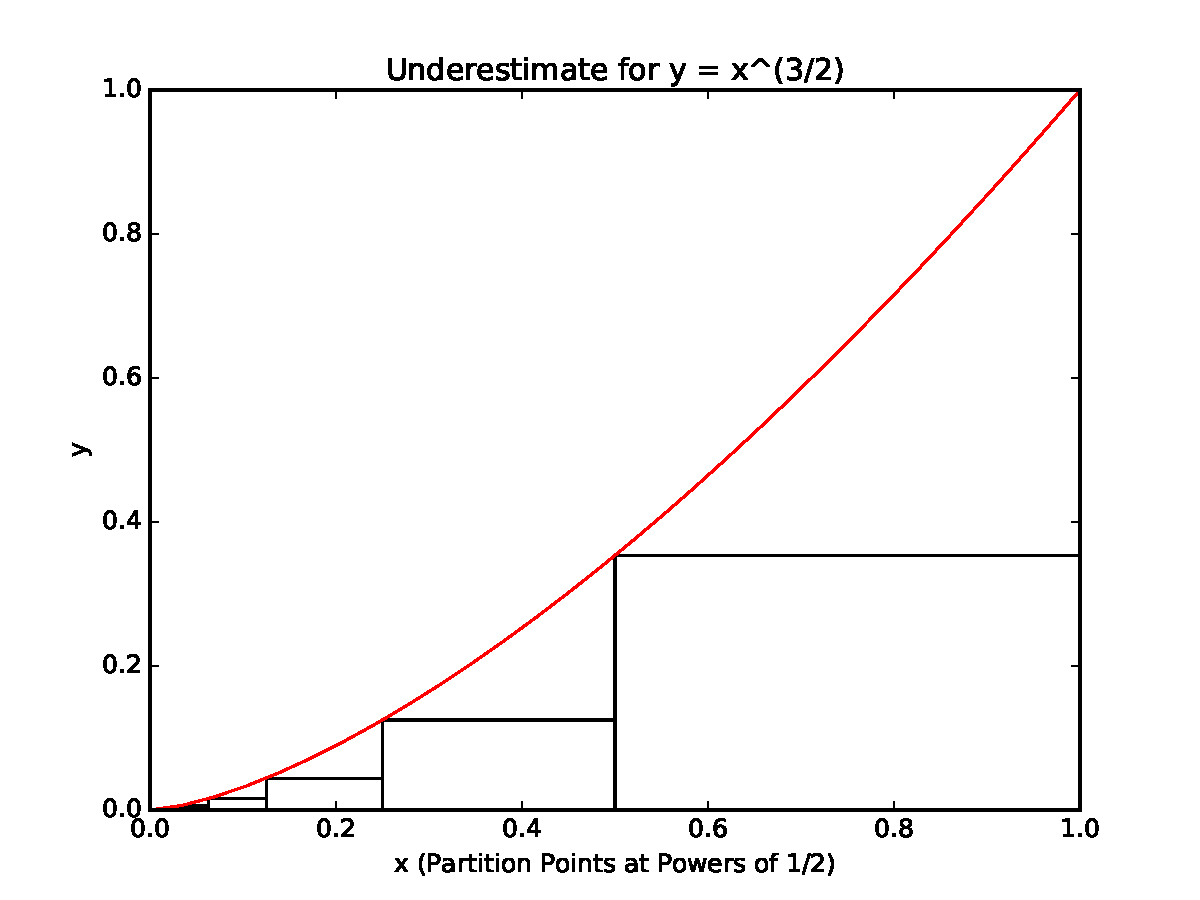
\includegraphics[width = 5in]{_generated/fermatLower.pdf}

The behavior of the rectangles is dictated by the following pattern:

\begin{itemize}
\item The rectangle of width \(1/2\) is from \(1/2 \leq x \leq 1\). 
\item The rectangle of width \(1/4\) is from \(1/4 \leq x \leq 1/2\).
\item The rectangle of width \(1/8\) is from \(1/8 \leq x \leq 1/4\). 
\item Etc...
\end{itemize}

The amazing consequence of Fermat's idea is that we can actually compute the area of these infinite number of rectangles since their areas turn out to be a geometric series.
Recall that a geometric sum is of the form \(b + b^2 + ... + b^n\) for some base \(b\) and power \(n\); this can be expressed more explicitly as
\begin{equation}
b + b^2 + ... + b^n = \frac{b - b^{n+1}}{1 - b}.
\end{equation}
So for bases \(b\) satisfying \(|b| < 1\), we get an expression for the infinite series:
\begin{equation}
b + b^2 + b^3 + ... = \frac{b}{1 - b}.
\end{equation}
Let us see how this is related to the area of the rectangles described above.

The area of the rectangles are:
\begin{itemize}
\item The area of the rectangle on \(1/2 \leq x \leq 1\) is \( (1/2)^{3/2} (1/2) = (1/2)^{5/2}\).
\item The area of the rectangle on \(1/4 \leq x \leq 1/2\) is \( (1/4)^{3/2} (1/4) = (1/4)^{5/2}\).
\item The area of the rectangle on \(1/8 \leq x \leq 1/4\) is \( (1/8)^{3/2} (1/8) = (1/8)^{5/2}\).
\item Etc.
\end{itemize}

So we have that the total area is 
\begin{equation}
(1/2)^{5/2} + (1/4)^{5/2} + (1/8)^{5/2} + ... 
    = (1/2)^{\frac{5}{2}} + \left((1/2)^{\frac{5}{2}}\right)^2 + \left((1/2)^{\frac{5}{2}}\right)^3 + ... 
\end{equation}
So we have an infinite geometric series with base \(b = (1/2)^{\frac{5}{2}}\). Therefore, this set of an infinite rectangles gives us a lowerbound
of \(\frac{(1/2)^{5/2}}{1 - (1/2)^{5/2}}\) for the area under \(y = x^{3/2}\) and \(0 \leq x \leq 1\).

A similar argument can be applied to another set of rectangles whose widths are powers of \(1/2\), as pictured below:

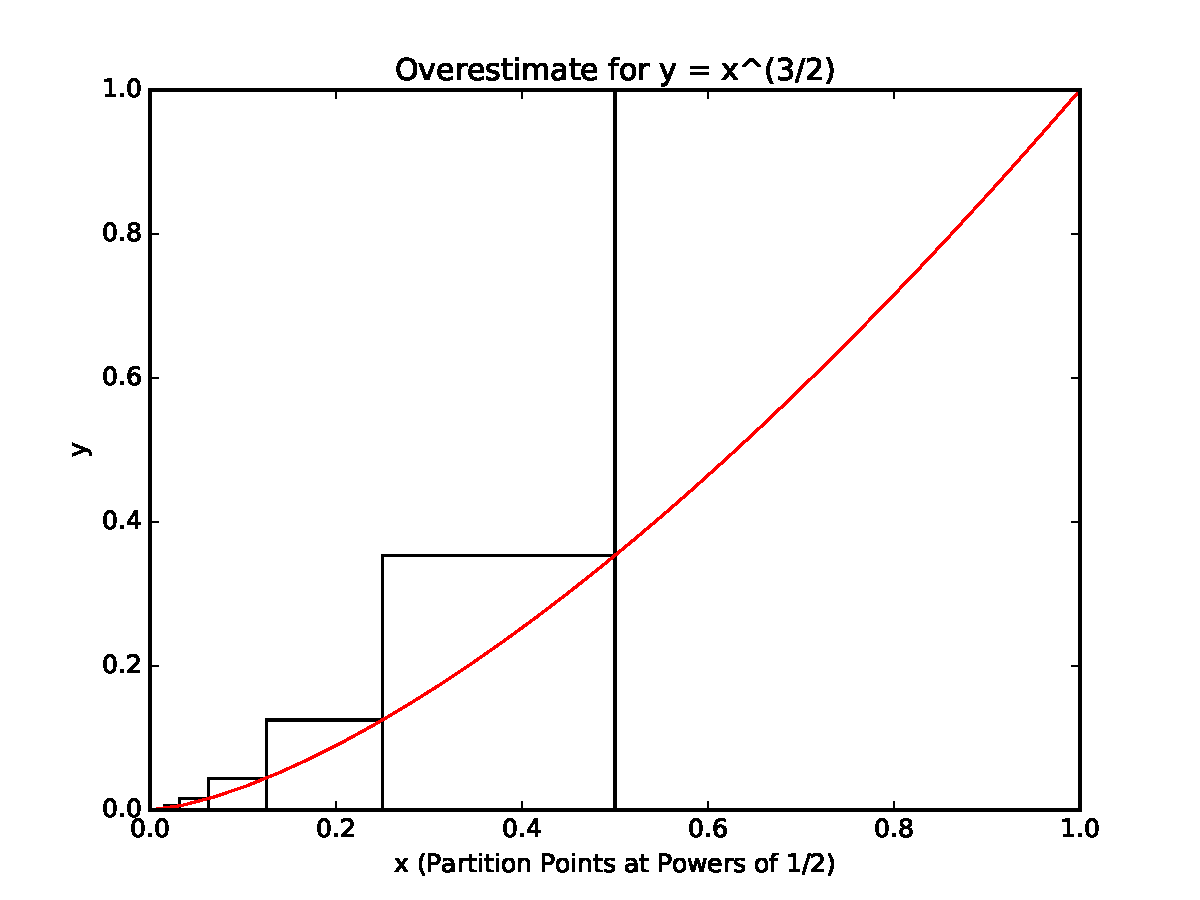
\includegraphics[width = 5in]{_generated/fermatUpper.pdf}

The final part of Fermat's idea is to do the above for general base \(0 < b < 1\). Then we consider the limit as \(b \to 1\).

\subsubsection*{The Problem}

Use Fermat's method to find the area under the curve \(y = x^{\frac{3}{2}}\) and \(0 \leq x \leq 1\).

\subsubsection*{The Solution}

Let us first construct the lower bound using rectangles whose widths are powers of a fixed base \(b\) satisfying \(0 < b < 1\). 
Similar to the case of base \(1/2\) we discussed before, we have that the rectangles satisfy
\begin{itemize}
\item There is a rectangle on \(b \leq x \leq 1\) of height \(b^{\frac{3}{2}}\).
\item There is a rectangle on \(b^2 \leq x \leq b\) of height \(\left(b^2\right)^{\frac{3}{2}}\).
\item There is a rectangle on \(b^3 \leq x \leq b^2\) of height \(\left(b^3\right)^{\frac{3}{2}}\).
\item Etc...
\end{itemize}
These rectangles have areas (repectively) \((1 - b)b^{\frac{3}{2}}\), \((1 - b) b\left(b^{\frac{3}{2}}\right)^2\), \((1-b)b^2\left(b^{\frac{5}{2}}\right)^3\), ...
So we see that the total area of these rectangles (and hence our lowerbound) is:
\begin{align}
(1 - b)b^{\frac{3}{2}} + (1 - b) b\left(b^{\frac{3}{2}}\right)^2 + (1-b)b^2\left(b^{\frac{5}{2}}\right)^3 + ... 
    & = \frac{1 - b}{b} \left( b^{\frac{5}{2}} + \left(b^{\frac{5}{2}}\right)^2 + \left(b^{\frac{5}{2}}\right)^2 + ...\right), \\
    & = \frac{1 - b}{b} \frac{b^{\frac{5}{2}}} {1 - b^{\frac{5}{2}}}, \\
    & = b^{\frac{3}{2}} \frac{1 - b}{1 - b^{\frac{5}{2}}}.
\end{align}
Now we use the algebraic fact that we can factor \(1 - y^2 = (1  - y) (1 + y)\) and \(1 - y^5 = (1 - y)(1 + y + y^2 + y^3 + y^4)\) for \(y = b^{\frac{1}{2}}\) to get that the lower bound is given by
\begin{equation}
b^{\frac{3}{2}} \frac{1 + b^{\frac{1}{2}}}
    {1 + b^{\frac{1}{2}} + b^{\frac{2}{2}} + b^{\frac{3}{2}} + b^{\frac{4}{2}}}.
\end{equation}

This lower bound is valid for all \(0 < b < 1\). So taking the limit as \(b \to 1\) we get a lower bound of
\begin{equation}
\frac{1 + 1}{1 + 1+ 1+ 1 + 1} = \frac{2}{5}.
\end{equation} 

We can use a similiar process to find an upper bound of \(\frac{2}{5}\). Since the upper bound and lower bound are the same, we must have that they are exaclty equal to the area.

Therefore, the area under \(y = x^{3/2}\) from \(0 \leq x \leq 1\) is \(\frac{2}{5}\).
